% VERWENDET !!
Eine Web Anwendung ein Programm, welches auf einem Server lauft und durch einen Web-Browser kundenseitig abgerufen wird, so \textcite[1]{mahmoud2017}.

% VERWENDET !!
Der Ablauf um einen solchen Code in die Anwendung injezieren zu können ist immer der Selbe, so \textcite{mahmoud2017}.
\begin{enumerate}
	\item Der Angreifer muss eine Schwachstelle in der Anwendung finden um seinen schadhaften Code in die Anwendung zu bringen und somit in weiterem Verlauf sensible Daten von seinem Opfer stehlen zu können.
	\item Das Opfer besucht die beschädigte Anwendung.
	\item Die Anwendung sendet eine Anfrage mit dem fehlerhaften Code im Body an einen Server.
	\item Wenn das Skript im Web-Browser des Opfers ausgeführt wird, kann der Angreifer diverse persönliche Informationen stehlen.
\end{enumerate}

% VERWENDET !!
\begin{figure}[ht]
	\centering
	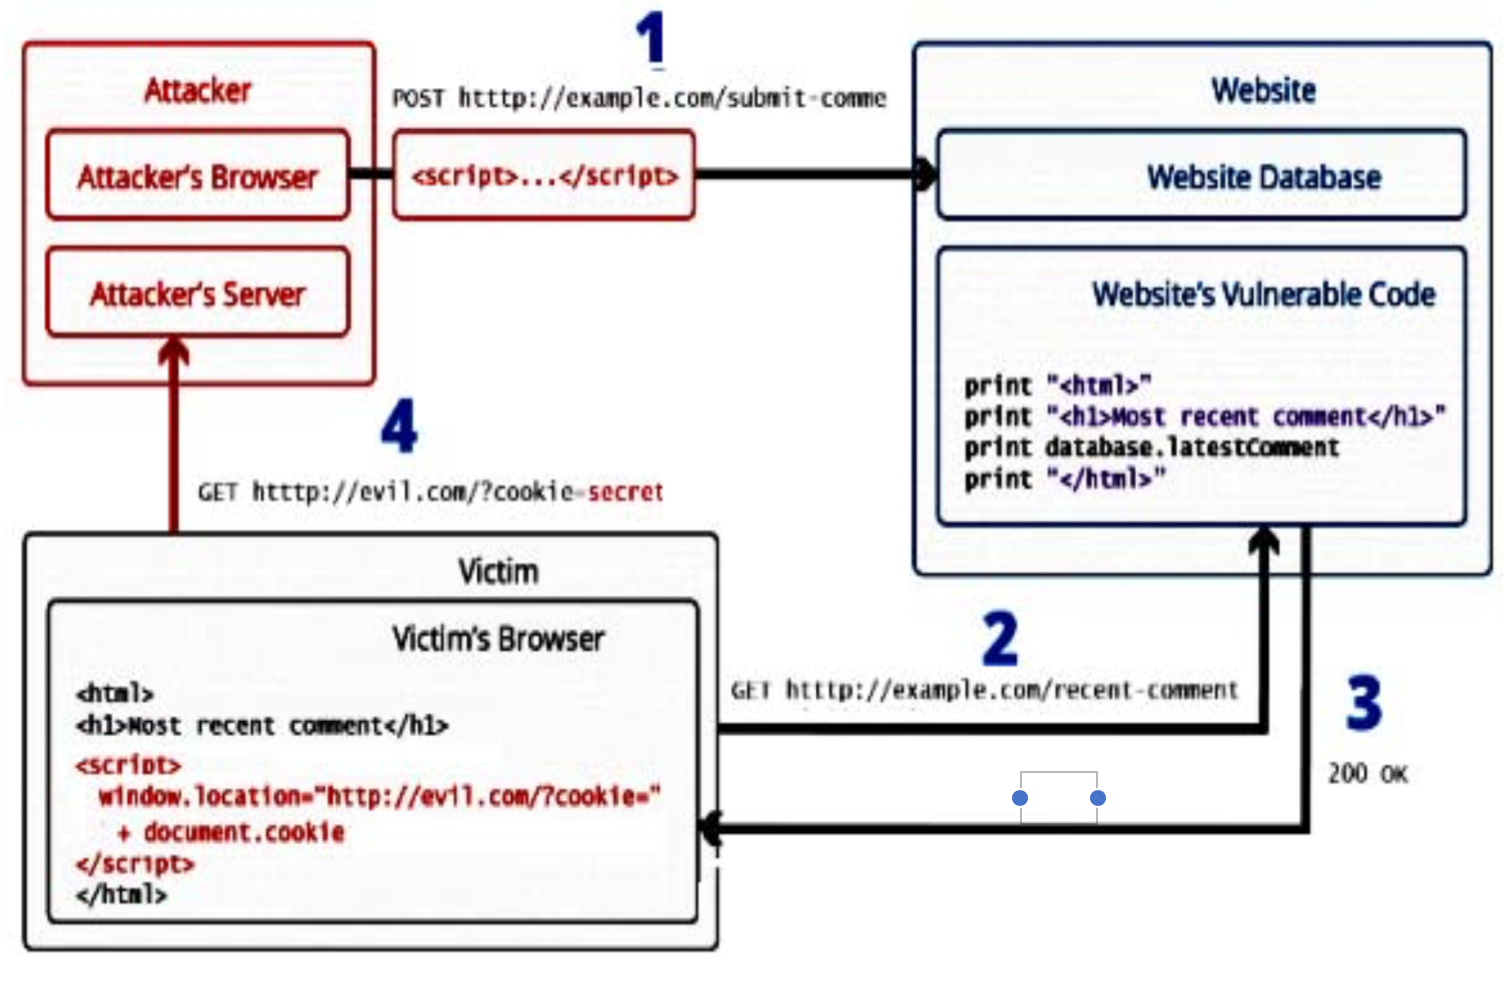
\includegraphics[width=0.75\linewidth]{images/XSS-attack-process.png}
	\caption{XSS Angriffsprozess\autocite[p]{mahmoud2017}}
\end{figure}


% VERWENDET !!
% FIXME: reflected XSS
Die Absicht von einer "reflected" XSS Attacke ist es sogenannte Session Cookies \footnote[]{http://www.allaboutcookies.org/cookies/session-cookies-used-for.html} vom Opfer zu stehlen. Diese Art von XSS Attacke benötigt stärkere Interaktion zwischen Opfer und Angreifer. Folgende Schritte müssen laut \textcite[2]{mahmoud2017} eingehalten werden und diese Attacke erfolgreich durchführen zu können.
% VERWENDET !!
Der Angreifer sendet seinem Opfer eine anfangs unscheinbare E-Mail mit einem Link. Dieser Link enthält einen schadhaften JavaScript Code, welcher ausgeführt wird, sobald das Opfer auf diesen klickt. Jetzt wird dieser vorhin platzierte Code an den Server geschickt, ohne dabei von der Web-Anwendung oder der Webseite entdeckt zu werden. In der Antwort des Servers wird dieser Code dem Opfer mitgesandt um somit im weiteren Verlauf die Session Cookies vom Opfer an die Domain des Angreifers zu übermitteln. Der Angreifer kann diese Cookies speichern und in Zukunft immer wieder verwenden.\autocite[2]{mahmoud2017}


% FIXME: stored XSS
Diese Art von XSS Attacke tritt regelmäßig in sozialen Netzwerken und anderen ähnlichen Web-Anwendungen auf. \textcite[2]{mahmoud2017} nennt diese Schritte um eine Schwachstellen einer XSS Attacke auszunutzen und umzusetzen.

Anders als bei der reflected XSS Attacke wird hierbei der schadhafte Code direkt in die Web-Anwendung oder die Webseite injeziert. Macht der Nutzer nun eine HTTP Anfrage auf den geschädigten Server, so wird der schadhafte Code als Antwort vom Server an das Opfer geschickt und im Web-Browser ausgeführt. Dieses sendet wiederum die Session Cookies des Opfers an die Domain des Angreifers, welcher diese dann dort speichern kann.